\documentclass[spanish]{article}
\usepackage[T1]{fontenc}
\usepackage[utf8]{inputenc}

\normalsize

\parindent = 0mm 

\usepackage{lmodern}
\usepackage[a4paper]{geometry}
\usepackage[spanish]{babel}
\usepackage{graphicx}
\usepackage{url}
\usepackage{booktabs}
\usepackage{multicol}
\usepackage{multirow}
\usepackage[x11names,table]{xcolor}
%\usepackage{float}
\usepackage{amsmath, latexsym, amsfonts, amssymb} 
\usepackage{multicol}
\usepackage[shortlabels]{enumitem}
\usepackage{tikz}
\usepackage{floatrow}
\usepackage[small,bf,labelsep=period]{caption}
\usepackage[backend=biber]{biblatex}

\bibliography{referencias}

\title{Proyecto Final Sistemas de Recuperación de Información}

\author{Lauren Guerra Hernández \and Dennis Fiallo Muñoz \and Paula Rodríguez Pérez}

\begin{document}

\maketitle

\section*{Presentación Visual}
	La interfaz visual se implementa usando las facilidades del módulo de Python \texttt{streamlit}. De esta se presentan a continuación sus funcionalidades.\\

	Presenta a su izquierda una barra de opciones como se ve en la imagen.

	\begin{multicols}{2}
		\begin{figure}[H]
			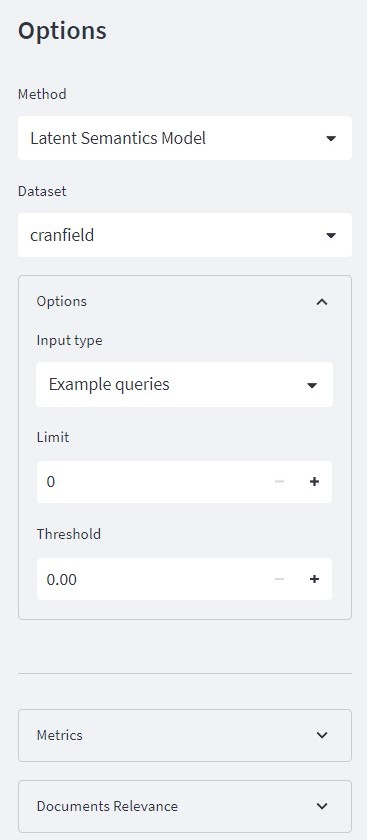
\includegraphics[scale=0.5]{visual.jpg}
		\end{figure}	
	
		Aparece primeramente un \texttt{selectbox} para alternar entre los modelos de recuperación de información presentados.\\

		Luego aparece otro \texttt{selectbox} para seleccionar el set de datos del cual se quiere hacer la consulta.\\

		Más abajo se presenta una ventada desplegable con las opciones de alternar el método para recibir la entrada de la consulta (entre una entrada de texto clásica o un conjunto de consultas predeterminado). Además, se puede cambiar tanto el límite como el umbral de los resultados que se devuelven.\\

		Bajo la línea va a estar una ventana desplegable que cuando se tengan los resultados de la consulta nos dará los resultados de las métricas.\\

		Mientras que más abajo se podrán ver de la consulta actual los documentos que son realmente relevantes, cuan relevantes con en realidad además de decir si este fue recuperado por el modelo seleccionado o no.\\
	\end{multicols}
		
		

		Mientras, del lado derecho de esta barra se mostrará la selección de consulta y los resultados de esta en ventanas desplegables en las cuales se da es título del documento, su contenido y su similitud con la consulta.

		\begin{figure}[H]
			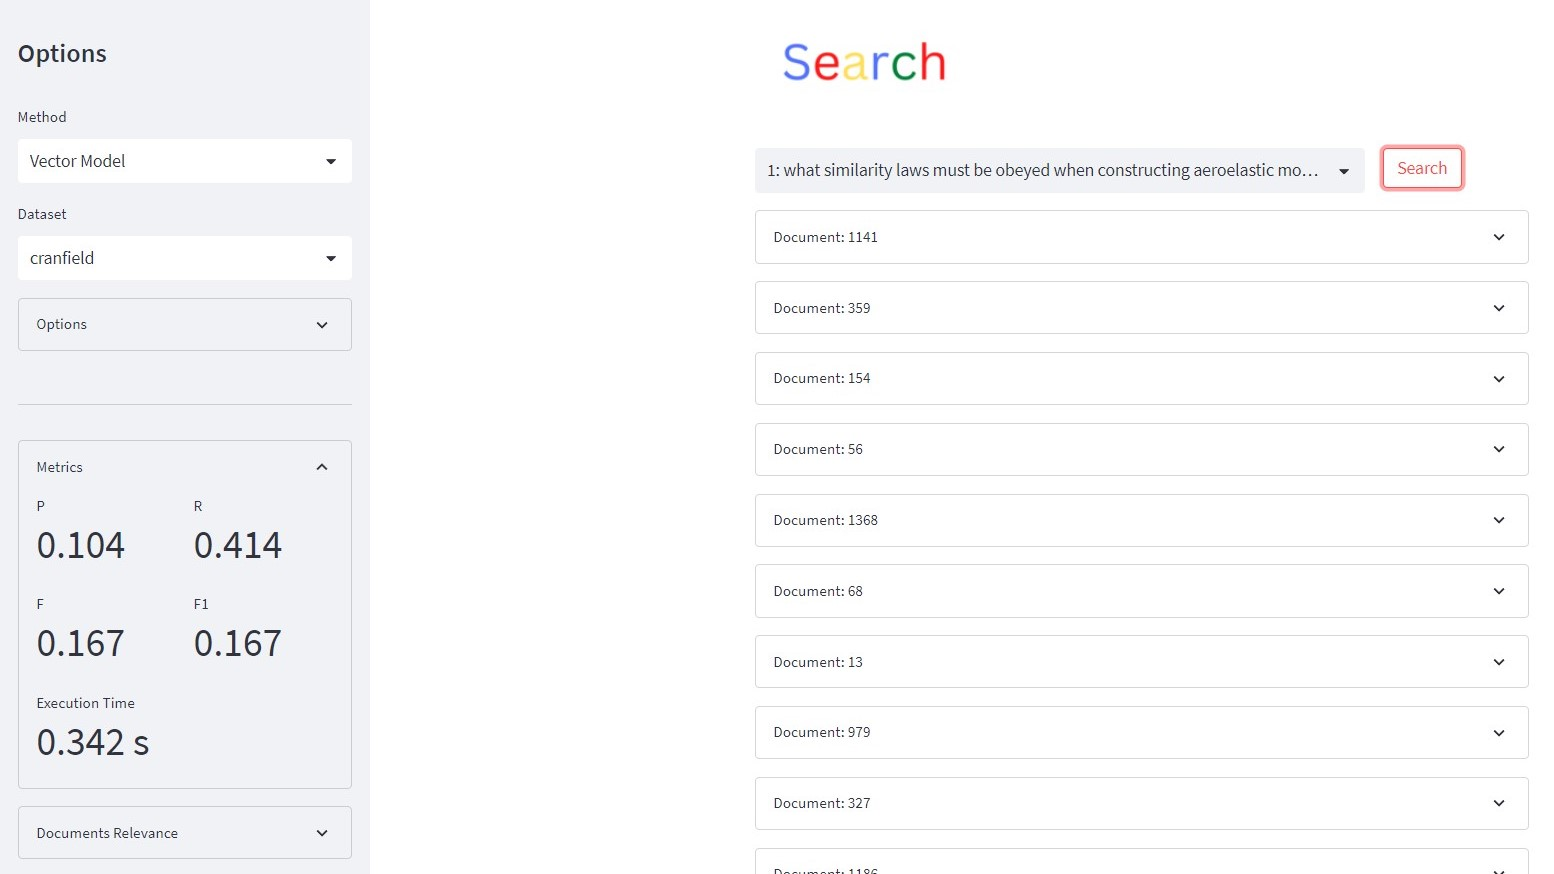
\includegraphics[scale=0.38]{visual_ex.jpg}
		\end{figure}
		
	\section*{Modelo Base}
		La implementación de los tres sistemas que presentamos van a seguir los mismos pasos en la recuperación de información pues heredan de la clase \texttt{base Model}. Por tanto, los sistemas van a seguir las etapas que se presentan a continuación:

			\begin{itemize}
				\item \textbf{Etapa 1:} Verificar si ya se tienen almacenada la información recuperada del set de datos actual, en caso de que no se hayan recuperado los datos de estos documentos con anterioridad se pasa a la Etapa 2 para extraer los datos, sin embargo, si ya se tienen los datos recuperados se pasa a la Etapa 5 para lograr mayor velocidad al mostrar los resultados ya que se cuenta con la información necesaria de los documentos.

				\item \textbf{Etapa 2:} Tomar los documentos del set de datos.

				\item \textbf{Etapa 3:}  Separar los términos de cada documento y eliminar los signos de puntuación y las \emph{stopwords}, luego se \emph{lexemizan} los términos para quedarnos con su forma canónica. Después de tener la lista de términos se pasa a aplicar la expansión de consulta buscando sinónimos del término y agregándolo a la consulta.

				\item \textbf{Etapa 4:} Calcular y almacenar la relación entre término con los documentos en que que aparece (cada modelo define su modo de hacer esta etapa).

				\item \textbf{Etapa 5:} Calcular y almacenar los pesos de las consultas en los documentos del siguiente modo: {término: w, ...}

				\item \textbf{Etapa 6:} Calcular la similitud de la consulta con los documentos usando los datos recopilados anteriormente.

				\item \textbf{Etapa 7:} Devolver \emph{ranking} de documentos.

			\end{itemize}	

	\section*{Implementación del código y herramientas usadas}
		
		
		El código va a tener separado en diferentes archivos las clases principales de la ejecución que serían:\\

		\texttt{Model}: Este se encuentra en \texttt{base\_model.py} y será la base de todos los modelos de recuperación de información que se presentan.\\

		\texttt{Datasets}: Aparece en \texttt{dataset.py}, este se va a inicializar desde \texttt{Model}. Se encarga de extraer la información de los \texttt{datasets}; desde los términos en los documentos, hasta las consultas de ejemplo y la relevancia real de los documentos con respecto a las consultas. Además, tiene un conjunto de propiedades y métodos estáticos para tomar datos necesarios en diferentes formas según el uso que se le va a dar. Se apoya en el módulo de python \texttt{ir\_datasets} para facilitar el acceso a la información de los \texttt{datasets} de ejemplo.\\

		\texttt{Lexemizer}: Este se encuentra en \texttt{lexemizer.py}. Apoyándose de las facilidades del módulo \texttt{nltk}, este está destinado a normalizar los términos de los documentos y de las consultas; separando las palabras en \emph{tokens} independientes, eliminado las \emph{stopwords}, eliminando las mayúsculas y \emph{lematizando} los términos, y para el caso de las consultas también se le aplica una expansión de consulta usando \texttt{wordnet} para agregar sinónimos de los términos.\\

		Visual: Se encuentra en \texttt{visual.py} y se encarga de llevar todo el proceso visual del proyecto.
	
	\section*{Modelo Vectorial}

		Como ya vimos anteriormente, la implementación del Modelo Vectorial va a heredar de la clase \texttt{Model}, siguiendo pasos similares al resto de modelos. En un principio, al inicializar el modelo se crean 3 \texttt{dict} vacíos, los cuales van a ser usados más adelante, siendo estos:\\

		\texttt{docterms}: un diccionario que tendrá como llaves los términos de todos los documentos, teniendo como \texttt{valid} almacenado cada uno los documentos en que aparecen y de estos la frecuencia, $ tf, idf $ y $ w $. Se usa esto pues la mayor parte de los términos aparecen en una pequeña parte de los documentos, por tanto, al eliminar los elementos que no son necesarios se puede lograr ahorrar algo de tiempo de procesamiento.\\

		\texttt{queryterms:} diccionario de términos de la \emph{query} con su respectivo peso.\\
		
		\texttt{querysim:} diccionario de documentos que tienen como valor su similitud con la consulta.\\

		Luego se siguen una serie de etapas que en general se siguen en todos los modelos. Se comienza verificando si ya se encuentran recopilados los datos de los términos de los documentos, en este caso en \texttt{docterms}, si se encuentra vacío se extrae la información apoyándose en la clase \texttt{Datasets}. Para los cálculos de estos datos se usan las formulas clásicas de:
			
		\begin{equation}
			\displaystyle tf_{ij} =  \frac{freq_{ij}}{max_l freq_{lj}}
		\end{equation}
		\begin{equation}
			\displaystyle idf_i =  log⁡{\frac{N}{n_i}}
		\end{equation}
		\begin{equation}
			\displaystyle w_{ij} = tf_{ij} \cdot idf_i
		\end{equation}

		Mientras que para la consulta se aplica un suavizado variable con valor predeterminado de 0.5:
		
		\begin{equation}
			\displaystyle w_{ij} = \left( \alpha + 
\left( 1 - \alpha \right) \frac{freq_{iq}}{max_l \ freq_{lq}} \right) log⁡ \frac{N}{n_i}
		\end{equation}

		De estos se tiene que:

		\begin{itemize}
			\item $ freq_{ij} $ sería la frecuencia del término $ t_i $ en el documento $ d_j $.

			\item Se calcula el máximo de los documentos.

			\item Si no aparece el término $ t_i $ en el documento $ d_j $ entonces $ tf_{ij} = 0 $.

			\item $ N $ es la cantidad de documentos en el sistema.

			\item $ n_i $ es es la cantidad de documentos en que aparece el término $ t_i $.
		\end{itemize}

		Luego de tener los datos de los términos en los documentos y de la E se pasa a calcular la similitud entre estos usando:
	
		\begin{equation}
			\displaystyle sim \left(d_j, q \right) = \displaystyle \frac{\displaystyle\sum_{i=1}^n (w_{ij} \cdot w_{iq})}{\sqrt{\displaystyle\sum_{i=1}^n w_{ij}^2} \ \sqrt{\displaystyle\sum_{j=1}^n w_{jq}^2}}
		\end{equation}

		Luego se devuelve un \emph{ranking} organizado por similitud y eliminando los que sean cero, o en caso de existir un umbral los que estén por encima de este.

		\section*{Modelo Probabilístico}

			La implementación del Modelo Probabilístico hereda de la clase \texttt{Model}. En la inicialización del modelo se tendrán 3 diccionarios (\texttt{dict}) y un conjunto (\texttt{set}): \\

			\texttt{term\_docs:} diccionario para almacenar los términos de la colección y su respectiva lista de documentos en los que aparece.\\

			\texttt{queryterms:} diccionario para almacenar los términos de la consulta.\\

			\texttt{query\_doc\_sim:} diccionario para almacenar por cada documento de la colección su similitud con la consulta.\\

			\texttt{term\_p\_r:} diccionario para almacenar las probabilidades de ocurrencia de un término en un documento relevante o no relevante a la consulta. Estas probabilidades serán almacenadas en una tupla donde el primer valor corresponde a la probabilidad de ocurrencia del término en un documento relevante a la consulta y en la segunda posición la probabilidad de que ocurra en un documento no relevante a la consulta.\\

			Al igual que en los otros modelos implementados se verifica si ya se analizó la ocurrencia de los términos de la colección en los documentos, en este caso en \texttt{term\_docs} es donde se almacena dicha información, si se encuentra vacío se extrae la información apoyándose en la clase \texttt{Datasets}.

			Para la implementación de nuestro modelo inicialmente la probabilidad de ocurrencia de un término en un documento relevante será tomada como una constante (0.5) y la probabilidad de ocurrencia de un término en un documento no relevante como:

			\begin{equation}\label{key}
				\displaystyle r_i = \frac{n_i}{N}
			\end{equation}

			Donde: 
			\begin{itemize}
				\item $ N $ es la cantidad de documentos en la colección.

				\item $ n_i $ es es la cantidad de documentos en que aparece el término $ t_i $.
			\end{itemize}

			Posteriormente con estos valores de probabilidades iniciales se procede a calcular la similitud entre un documento y la consulta a través de la siguiente fórmula:
	
			\begin{equation}
				\displaystyle sim(d_j,q) = \sum_{i=1}^m \left( w_{i,j} \cdot w_{i,q} \cdot log⁡ \ \frac{p_i (1 - r_i)}{(1- p_i ) r_i} \right)
			\end{equation}

			Donde:
			\begin{itemize}
				\item $ w_{i,j}, w_{i,q} $ son la ocurrencia del término $ i $ en el documento $ j $ y la consulta respectivamente.

				\item $ p_i, r_i $ serán las probabilidades de que el término $ i $ ocurra en un término relevante o no relevante respectivamente.
			\end{itemize}

			Una vez obtenidos estos valores de similitud se realizará un \emph{ranking} con los mismos. 

			Luego se procederá a realizar una pseudo-retroalimentación y para ello los valores de $ p_i, r_i $ serán calculados de la siguiente forma:

			\begin{equation}
				p_i = \frac{|V_i| + 0.5}{|V| + 1}
			\end{equation}
			
			\begin{equation}
				\displaystyle r_i = \frac{n_i - |V_i| + 0.5}{N - |V| + 1}
			\end{equation}
			
			Donde:

			\begin{itemize}
				\item $ V $ es el conjunto de documentos recuperados.
				\item $ V_i $ es el conjunto de los documentos recuperados en los que aparece el término $ i $.
			\end{itemize}

			Serán aplicadas constantes de suavizado en cada una de las fórmulas (0.5 en el numerador y 1 en el denominador) para evitar división por cero o logaritmos indeterminados.\\
			
			Una vez obtenidos los nuevos valores de $ p_i, r_i $ la similitud será computada nuevamente y se retornará un \emph{ranking} en base a esta.\\

			Este proceso donde se calculan nuevamente las probabilidades de ocurrencia de los términos en documentos relevantes o no, se analiza la similitud y se devuelve un \emph{ranking} se realizará en tres ocasiones. El último \emph{ranking} calculado será retornado como respuesta del algoritmo y se tendrá en cuenta para este si es establecido un umbral para la similitud.


\end{document}